In einem Höppler-Viskosimeter (siehe Abb. \ref{fig:aufbau}) sinkt eine Kugel durch einem mit einer Flüssigkeit befüllten Zylinder. Hier ist es destilliertes Wasser. Beim Befüllen des Zylinders mit der Flüssigkeit und der Kugel ist darauf zu achten, dass sich keine Luftblasen an der Kugel bilden. Die Kugel fällt nicht, sondern sie rutscht an der Innenwand des leicht schräg stehenden  Zylinders herab. Das ist wichtig, um das Anschlagen der Kugel an den Innenwänden und dadurch entstehende Turbulenzen zu verhindern. \\
Die Zeit, die die Kugel braucht, um zwei Markierungen im Abstand von \SI{10}{\centi\meter} zu passieren ist die Fallzeit. Diese wird für zwei verschieden große Kugeln zehn Mal bei Raumtemperatur gemessen. 
In einer zweiten Messreihe wird das destillierte Wasser erhitzt und die Fallzeit der größeren Kugel bei zehn verschiedenen Temperaturen je zwei Mal gemessen. \\
Beide Kugeln werden vor Versuchsbeginn vermessen und gewogen. \\

\begin{figure}[h!]
	\centering
	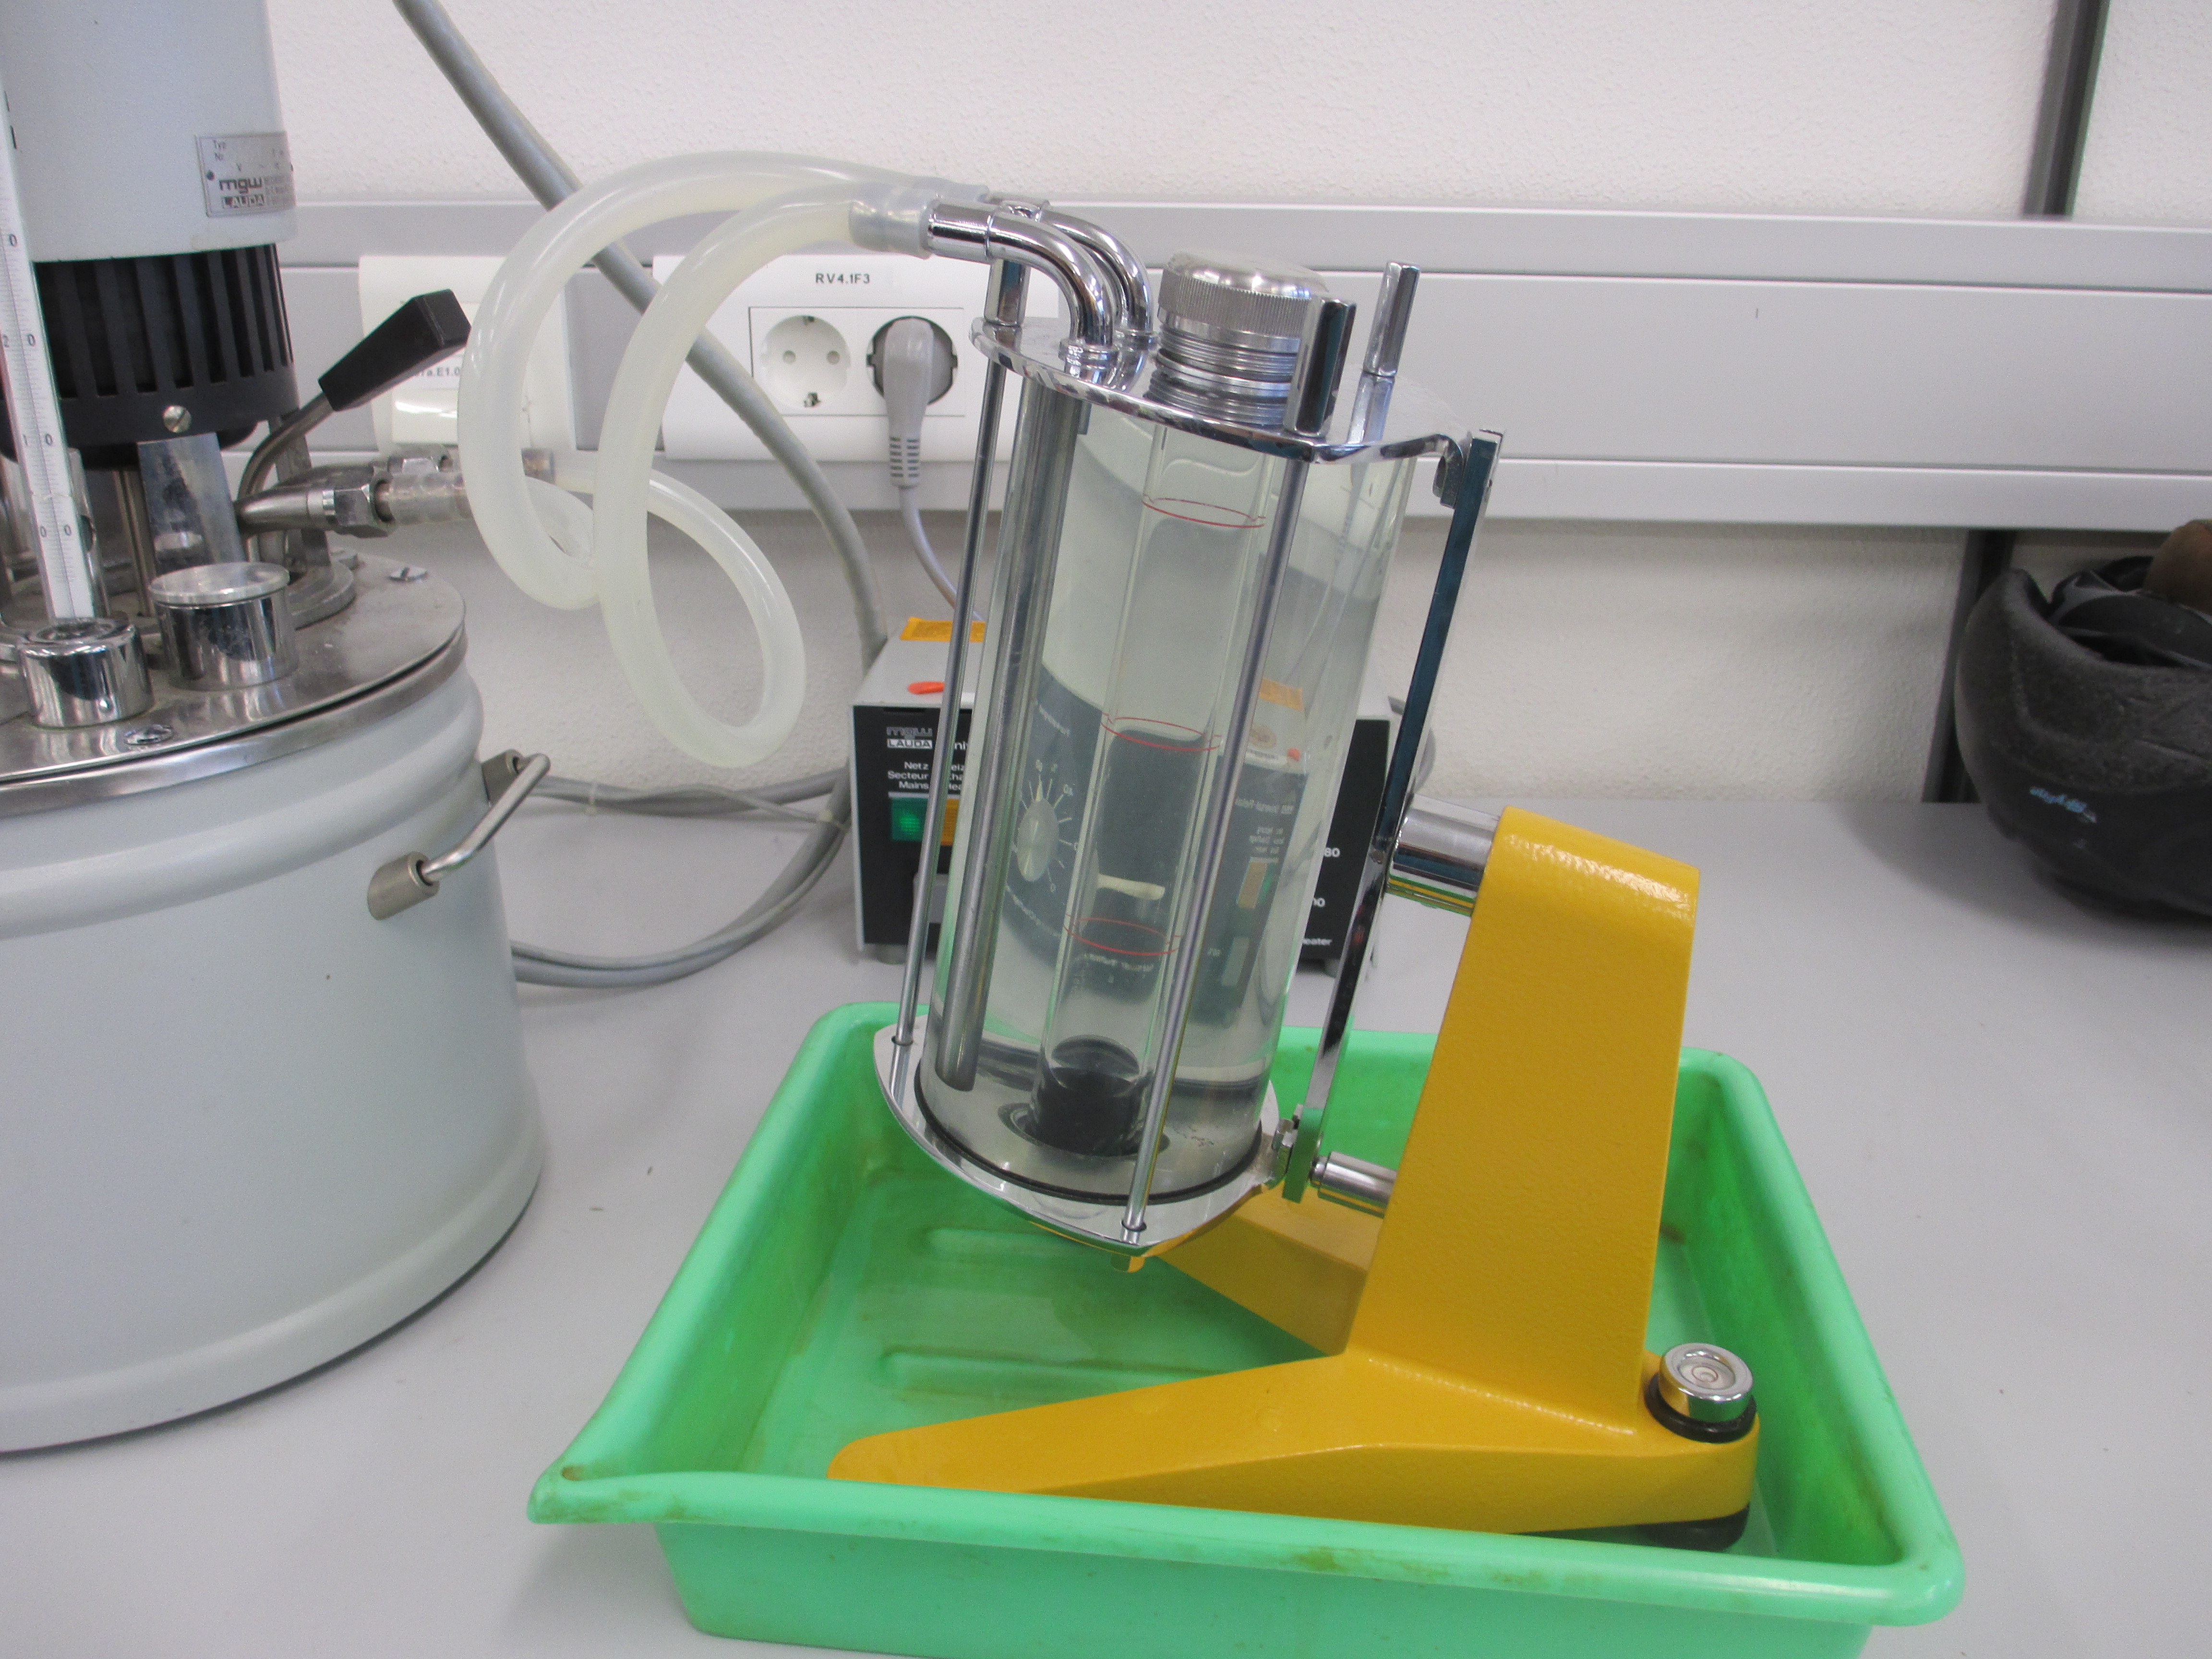
\includegraphics[width=0.5\textwidth]{Versuchsaufbau.JPG}
	\caption{Höppler-Viskosimeter mit Heizung}
	\label{fig:aufbau}
\end{figure}

\todo[color=red, inline]{Das ist alles super kurz, aber was haben wir denn sonst noch gemacht?!}
 
 